\documentclass[13pt,a4paper]{article}

\usepackage[utf8]{inputenc}
\usepackage{graphicx}
\usepackage{wrapfig}
\usepackage{color}
\usepackage{xcolor}
\usepackage{amsmath}
\usepackage{amssymb}
\usepackage[inkscapelatex=false]{svg}
\usepackage{array, makecell}
\usepackage{mhchem}
\usepackage{tabularx}
\usepackage{svg}
\usepackage{braket}
\usepackage{listings}
\definecolor{commentsColor}{rgb}{0.497495, 0.497587, 0.497464}
\definecolor{keywordsColor}{rgb}{0.000000, 0.000000, 0.635294}
\definecolor{stringColor}{rgb}{0.558215, 0.000000, 0.135316}
\lstset{
    frame=single,
    language=Python,
    basicstyle=\ttfamily\vspace{1em},
}

\usepackage[T1]{fontenc}
\usepackage[utf8]{inputenc}
\usepackage[lf]{Baskervaldx} % lining figures
\usepackage[bigdelims,vvarbb]{newtxmath} % math italic letters from nimbus Roman
\usepackage[cal=boondoxo]{mathalfa} % mathcal from STIX, unslanted a bit
\renewcommand*\oldstylenums[1]{\textosf{#1}}

\usepackage{multicol}
\usepackage{colortbl}
\usepackage[Export]{adjustbox}
\adjustboxset{max size={0.9\linewidth}{0.9\paperheight}}
\usepackage[colorlinks=true,linkcolor=red,citecolor=green]{hyperref}

\textwidth=16cm
\textheight=23cm
\topmargin=-2cm
\oddsidemargin=0cm
\setlength{\parindent}{0em}
\setlength{\parskip}{0.6em}
\setlength{\jot}{12pt}
\renewcommand{\arraystretch}{1.4}
\renewcommand{\theadfont}{\bfseries}
\newcommand{\todo}[1]{\textcolor{red}{TODO: #1}}


\begin{document}
\title{
    \LARGE
    \textbf{SATFD - lab 02 report}
}
\author{
    \large
    Dawid Karpiński, 18.03.2024
}
\date{}
\maketitle

\section{Comparison of signals in time and frequency domain.}

In figure \ref{fig:comparison} one can see the generated plots of different signals in time and frequency domain. The signals include an infinite signal, a rectangular window, a finite signal (result of multiplying the infinite signal with the rectangular window), a non-rectangular window, and a smoothed finite signal (result of multiplying the infinite signal with the non-rectangular window).

The multiplication of two signals in the time domain results in the convolution of their frequency domain representations.

\begin{lstlisting}[caption={\textbf{Code snippet for generating the signals.}}]
N = 1000
A = 5
f = 10
fs = 1000

dt = 1 / fs
time = dt * np.arange(N)

infi = A * np.sin(2 * np.pi * f * time)
window = time[time < 5 / f]
rect = np.pad(np.full(window.size, 1), ((time.size - window.size) // 2))
nonrect = scipy.signal.windows.gaussian(N, std=1 / f * N)

spectrum = np.abs(spectrum) ** 2
freqs = np.fft.fftfreq(signal.size, 1 / fs)
\end{lstlisting}

\begin{figure}[ht!]
    \centering
    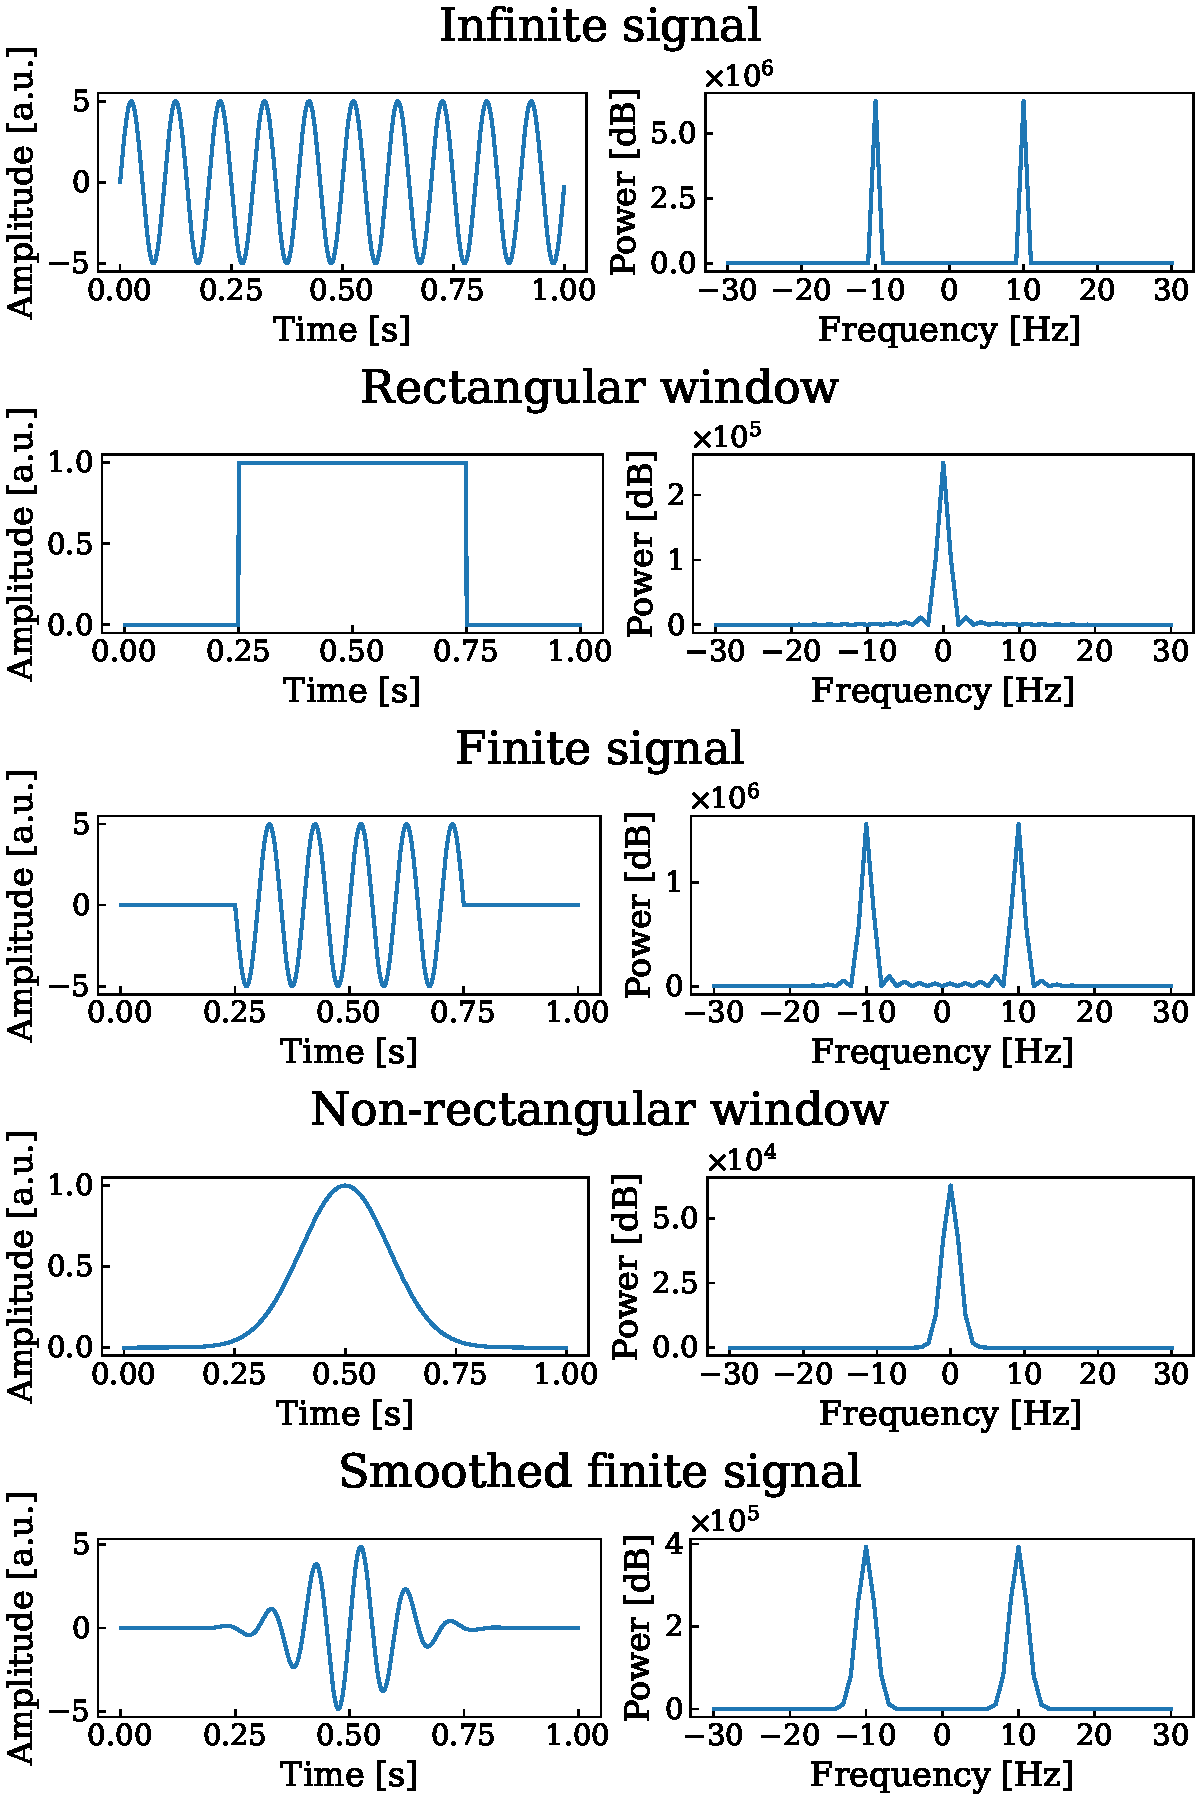
\includegraphics[width=0.9\linewidth]{spectra_comparison.pdf}
    \caption{\textbf{Signals comparison.}}
    \label{fig:comparison}
\end{figure}
\clearpage


\section{Sampling theorem and aliasing.}

According to the sampling theorem, to perfectly reconstruct a signal, the sampling frequency $f_s$ must be at least twice the maximum frequency of the signal. This minimum sampling frequency is called the Nyquist frequency.

The analysis has been performed on a Windows startup sound (figure \ref{fig:wave}), with the original sample rate of $f_s=22.05$ [kHz]. The following plots in figure \ref{fig:sampling_thorem} show a gradually decimated signal, with the removal of every other sample, where the impact of sampling frequency on the frequency domain representation of the signal can be observed.

\begin{figure}[ht!]
    \centering
    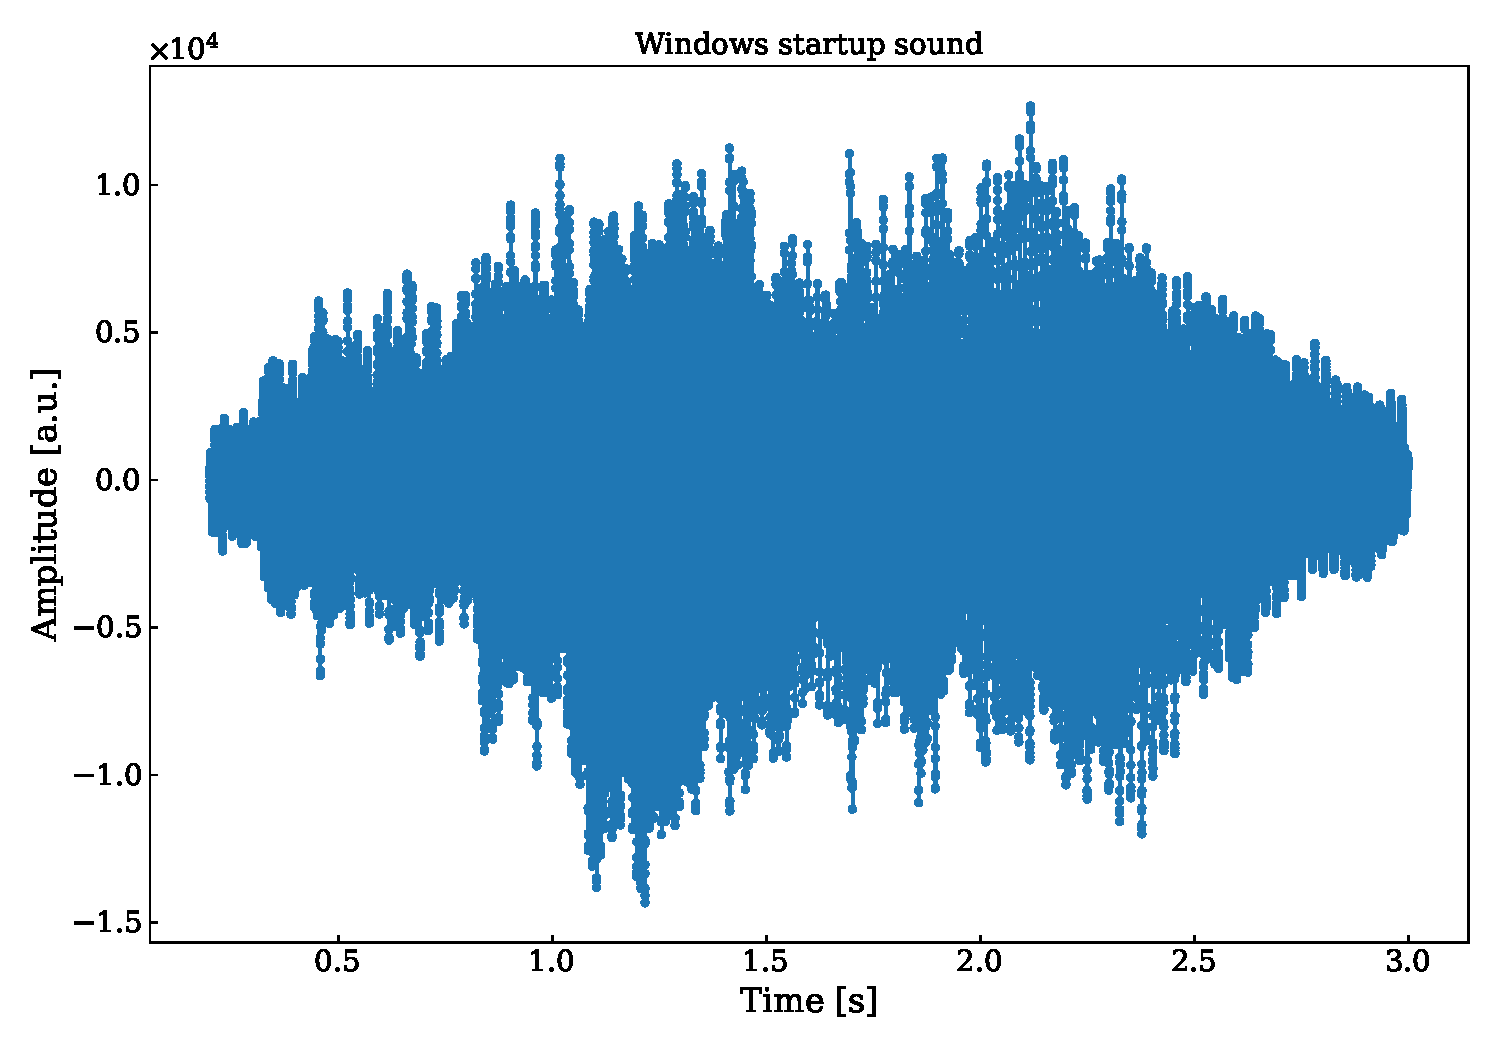
\includegraphics[width=\linewidth]{wave.pdf}
    \caption{\textbf{Windows startup sound.}}
    \label{fig:wave}
\end{figure}

At each decimation, the range of signal's frequencies moved towards larger values. Additionally, some of the frequencies are lost, probably due to occurring aliasing.

\begin{lstlisting}[caption={\textbf{Code snippet for gradual decimation of the signal.}}]
fss = fs // np.array([1, 1.5, 2, 5, 10])

for curr_fs in fss:
    samples = round(wave.size * curr_fs / fs)
    rwave, rtime = signal.resample(wave, samples, t=time)
\end{lstlisting}

\begin{figure}[ht!]
    \centering
    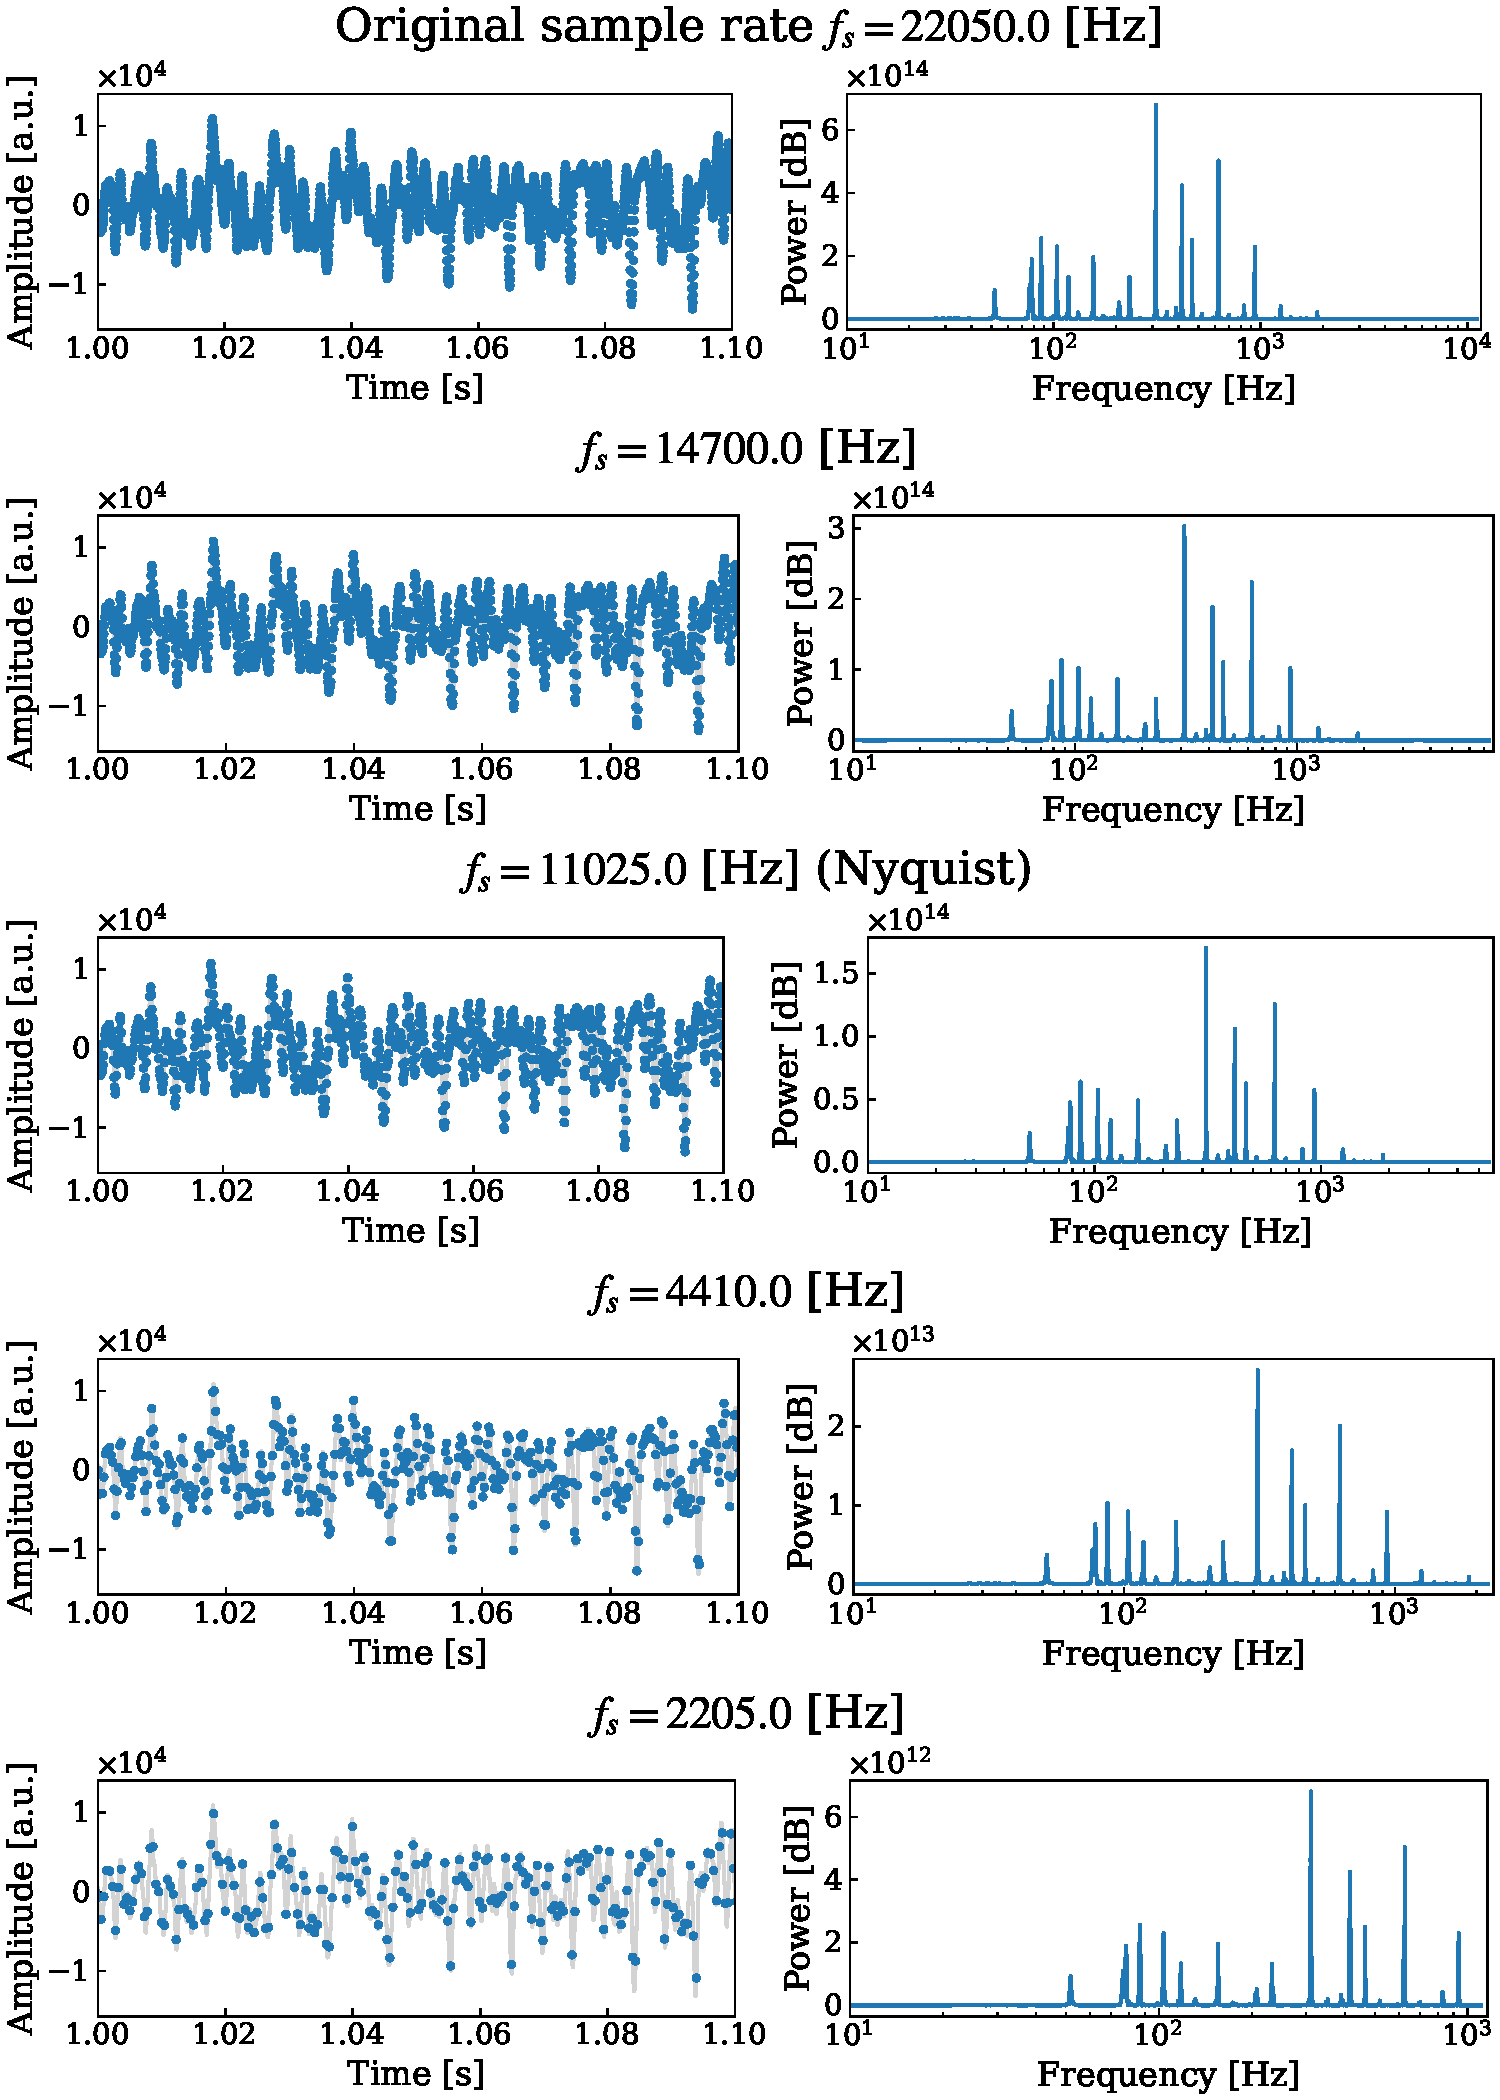
\includegraphics[width=\linewidth]{sampling_thorem.pdf}
    \caption{\textbf{Signals comparison. For better readability, only 0.1 [s] of the signal in the time domain is shown.}}
    \label{fig:sampling_thorem}
\end{figure}
\clearpage


\section{Zero-padding the signal.}

Zero padding is a technique used to increase the resolution of the frequency domain representation of a signal. The signal is therefore extended by adding zeros to its end, effectively increasing its length.

\begin{lstlisting}[caption={\textbf{Code snippet for adding the padding to infinite signal.}}]
wave = np.pad(wave, (0, wave.size * 3))
time = np.arange(wave.size) / fs
\end{lstlisting}

\begin{figure}[ht!]
    \centering
    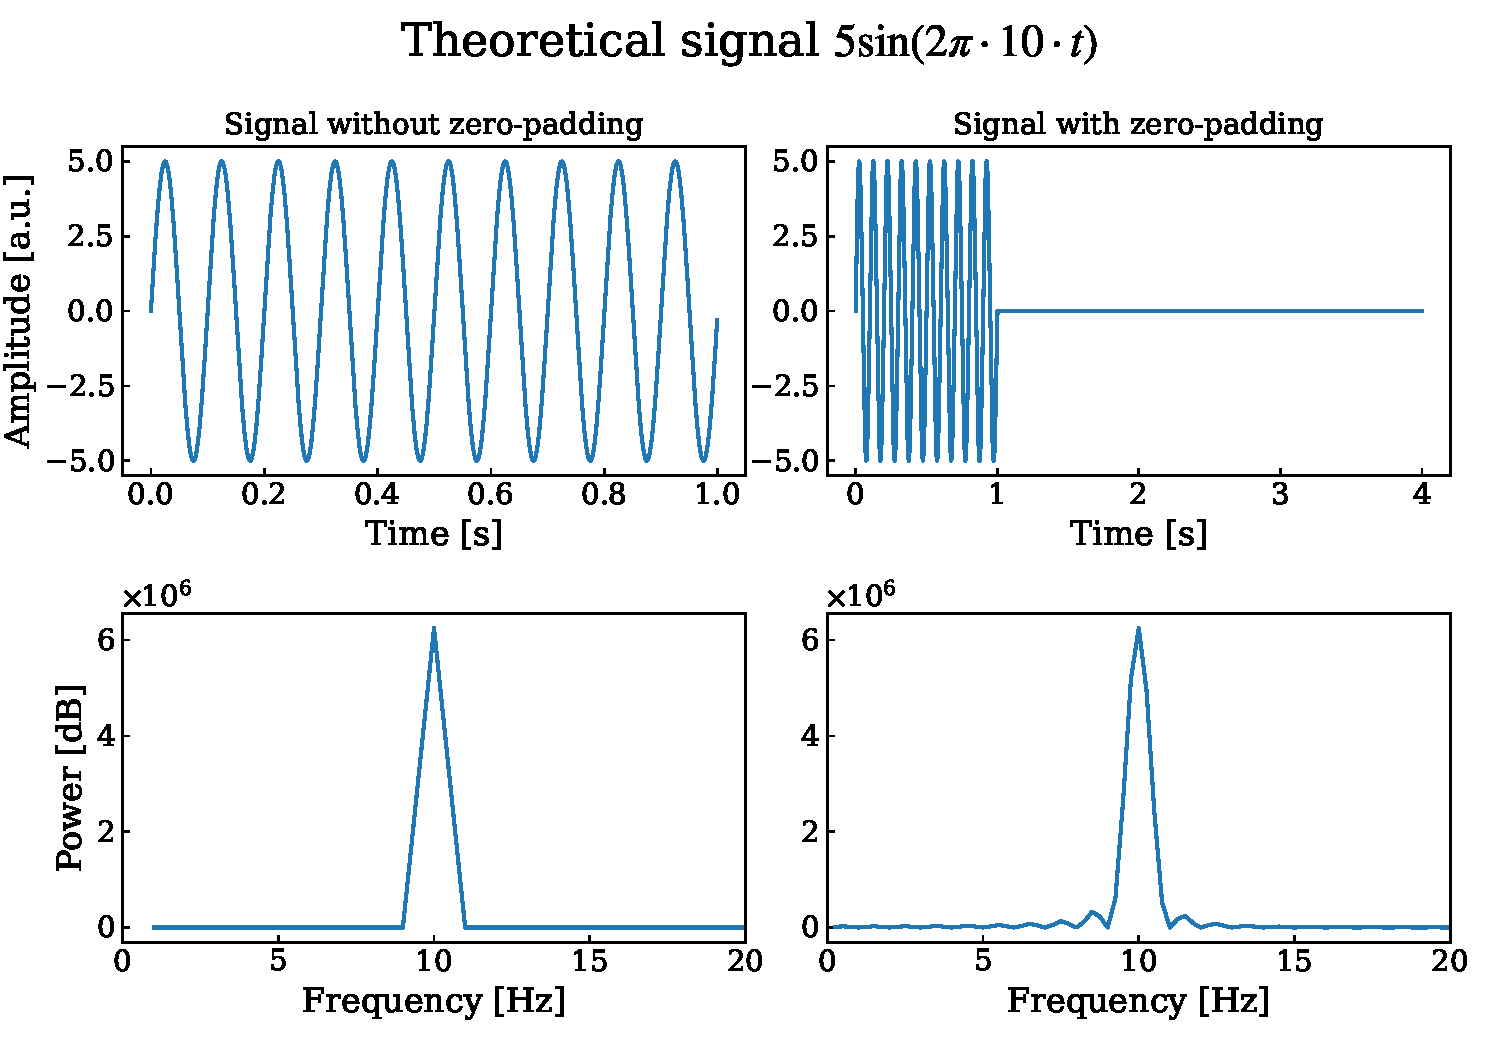
\includegraphics[width=\linewidth]{zero_pad.pdf}
    \caption{\textbf{Zero padding.}}
    \label{fig:zero_padding}
\end{figure}
\pagebreak


\section{Signal upsampling.}

In upsampling, the signal is interpolated by inserting zeros between the samples, which results in a higher sampling rate.

\begin{lstlisting}[caption={\textbf{Code snippet for upsampling the signal.}}]
upsampled = np.zeros(wave.size * 2)
upsampled[::2] = wave

new_fs = 2 * fs
time = np.arange(wave.size * 2) / new_fs
\end{lstlisting}

\begin{figure}[ht!]
    \centering
    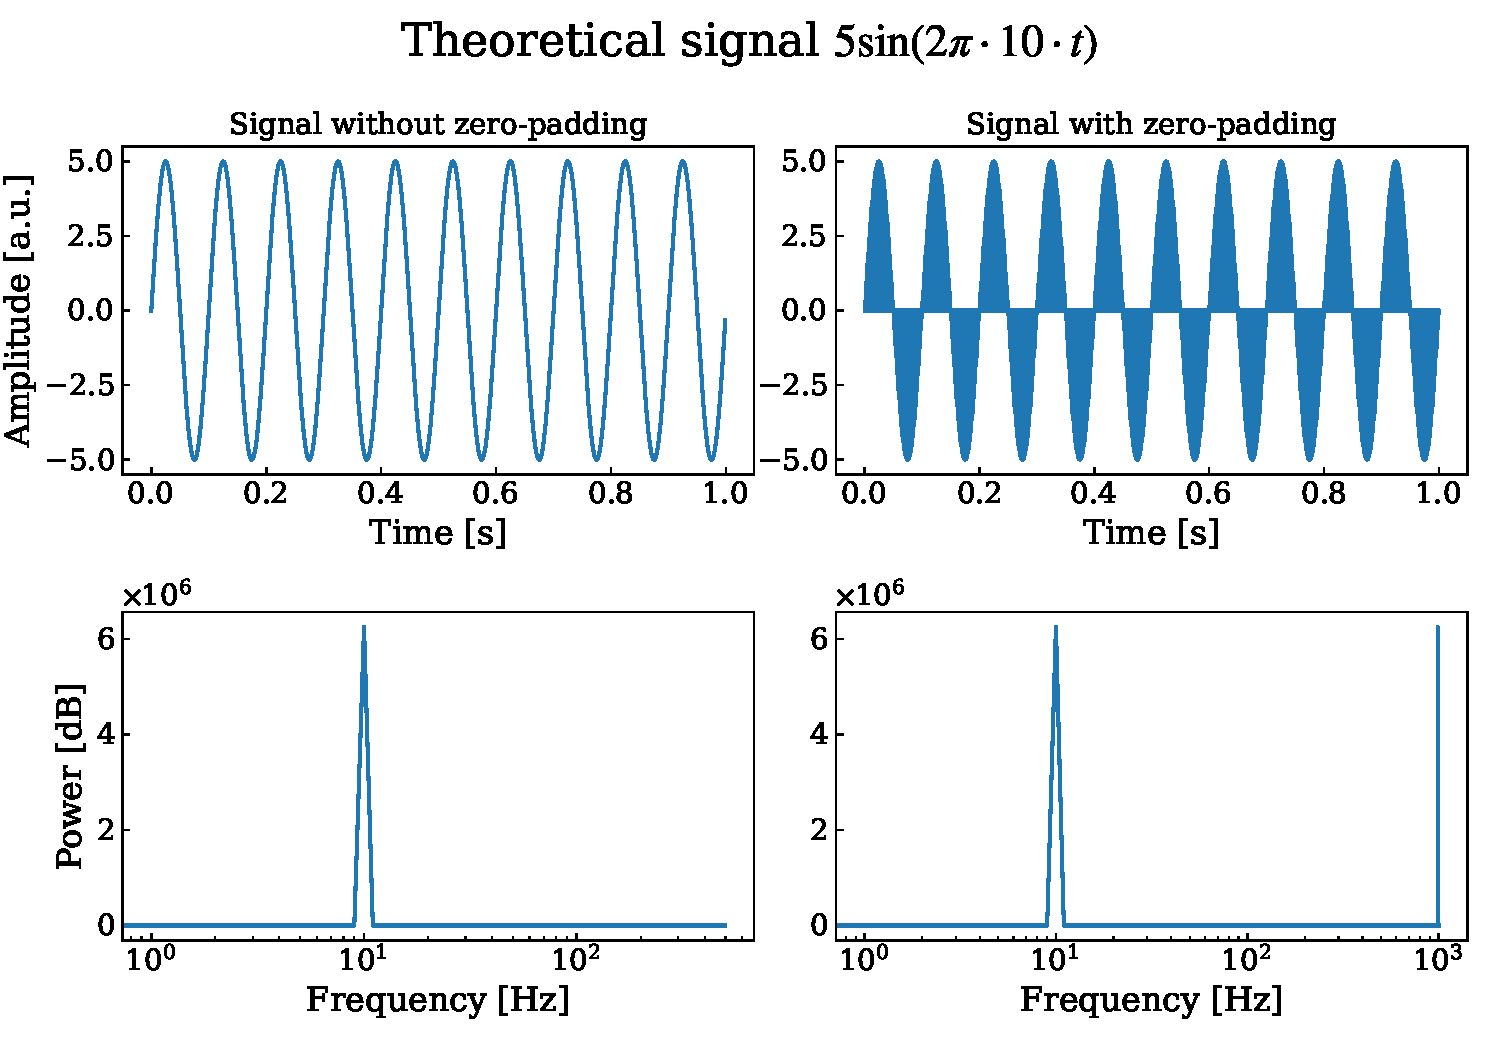
\includegraphics[width=\linewidth]{upsampling.pdf}
    \caption{\textbf{Signal upsampling.}}
    \label{fig:upsampling}
\end{figure}

Moreover, after performing the upsampling, a new frequency appeared in the power spectrum.


\pagebreak
\section{Conclusion.}

In conclusion, the task in lab 02 has explored various aspects of signal processing, including the comparison of windows applied to signals in both time and frequency domains, the application of the sampling theorem and its implications on aliasing, zero-padding techniques to enhance frequency resolution, and signal upsampling by zero interpolation.

The entire code for generating the data and plots can be found at:

\url{https://github.com/davkk/signal-analysis/tree/main/sat/lab02}

\end{document}
